\section{要求定義}
 ユーザがシステムに求める機能や動作を決定する。以下に要求定義をまとめた図\ref{usecase}を載せる。
\ref{usecase}では、ユーザがシステムに対して動作を行った際にどのような振る舞いをするか記載してある。ユーザは通常の買い物のようにカートに商品を出し入れすることができる。このときカート(RaspberryPi)が商品に関するデータを集める。解析システムでは画像から商品の特定やカゴDBへの操作を行う。この解析システムはサーバで動作する。カゴDBではカート内にある商品の管理を行う。ここで管理されている情報が最終的な決済システムで利用される。ユーザはカートを返却すると決済システムが動作し自動で決済システムが動作し顧客の所持金からカート内の商品合計金額がひかれる。

\begin{figure}[htbp]
\centering
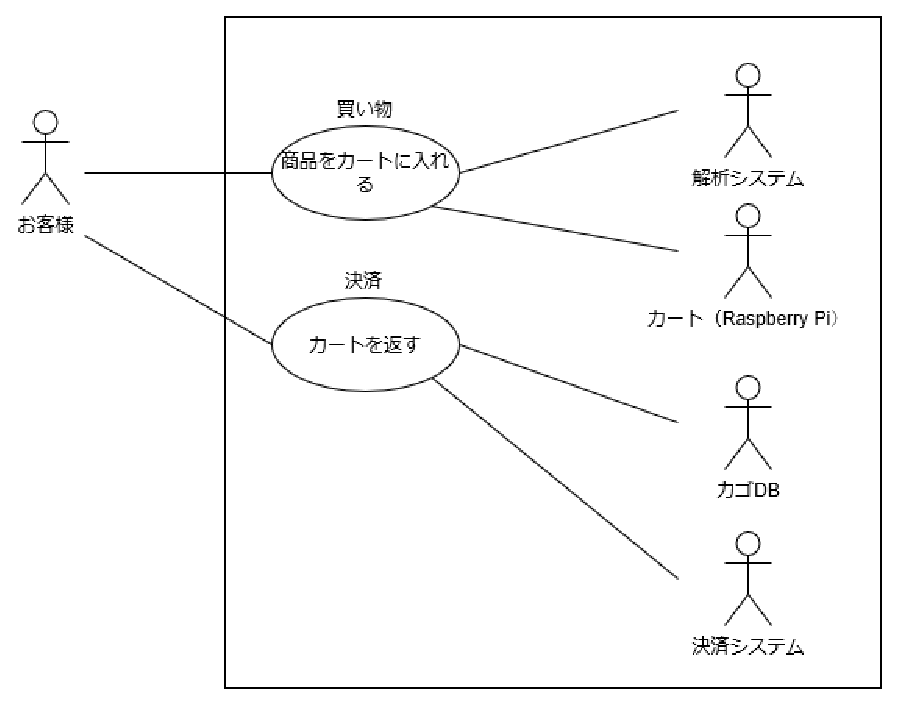
\includegraphics[width=12cm]{./pic/usecase_saishu.eps}
\caption{ユースケース図}
\label{usecase}
\end{figure}